%%%%%%%%%%%%%%%%%%%%%%%%%%%%%%%%%%%%%%%%%
% baposter Landscape Poster
% LaTeX Template
% Version 1.0 (11/06/13)
%
% baposter Class Created by:
% Brian Amberg (baposter@brian-amberg.de)
%
% This template has been downloaded from:
% http://www.LaTeXTemplates.com
%
% License:
% CC BY-NC-SA 3.0 (http://creativecommons.org/licenses/by-nc-sa/3.0/)
%
%%%%%%%%%%%%%%%%%%%%%%%%%%%%%%%%%%%%%%%%%

%----------------------------------------------------------------------------------------
%	PACKAGES AND OTHER DOCUMENT CONFIGURATIONS
%----------------------------------------------------------------------------------------

\documentclass[portrait,a0paper,fontscale=0.31]{baposter} % Adjust the font scale/size here

\usepackage[absolute,overlay]{textpos} % For absolute positioning
\usepackage{graphicx} % Para gráficos
\usepackage{multirow} % Para combinar celdas en varias filas
\usepackage{array}    % Para personalizar el formato de las columnas
\usepackage{enumitem}

\usepackage{graphicx} % Required for including images
\graphicspath{{figures/}} % Directory in which figures are stored

\usepackage{amsmath} % For typesetting math
\usepackage{amssymb} % Adds new symbols to be used in math mode

\usepackage{breqn}  % Used for breaking equations on multiple lines


\usepackage{booktabs} % Top and bottom rules for tables
\usepackage{enumitem} % Used to reduce itemize/enumerate spacing
\usepackage{palatino} % Use the Palatino font
\usepackage[font=small,labelfont=bf]{caption} % Required for specifying captions to tables and figures

\usepackage{multicol} % Required for multiple columns
\setlength{\columnsep}{1.5em} % Slightly increase the space between columns
\setlength{\columnseprule}{0mm} % No horizontal rule between columns

\usepackage{tikz} % Required for flow chart
\usetikzlibrary{shapes,arrows} % Tikz libraries required for the flow chart in the template

\usepackage{graphicx} % Required for including images and floating tables/figures
\usepackage{amsmath} % For advanced math formatting
\usepackage{amssymb} % For additional math symbols
\usepackage{float} % For the [H] specifier, which forces the table to be placed exactly where it appears in the code
\usepackage{booktabs} % For enhanced table formatting


%%%%%%%%%%
\usepackage{cite}
\usepackage{amsmath,amssymb,amsfonts}
\usepackage{algorithmic}
\usepackage{graphicx}
\usepackage{textcomp}
\usepackage{float}
\usepackage{xcolor}
\usepackage[spanish]{babel}
% \usepackage{hyperref}
%%%%%%%%%%

\newcommand{\compresslist}{ % Define a command to reduce spacing within itemize/enumerate environments, this is used right after \begin{itemize} or \begin{enumerate}
\setlength{\itemsep}{1pt}
\setlength{\parskip}{0pt}
\setlength{\parsep}{0pt}
}

\definecolor{lightblue}{rgb}{0.145,0.6666,1} % Defines the color used for content box headers

\definecolor{udesa}{RGB}{0, 18, 187} 

\begin{document}

\begin{poster}
{
headerborder=closed, % Adds a border around the header of content boxes
colspacing=1em, % Column spacing
bgColorOne=white, % Background color for the gradient on the left side of the poster
bgColorTwo=white, % Background color for the gradient on the right side of the poster
borderColor=udesa, % Border color
headerColorOne=udesa, % Background color for the header in the content boxes (left side)
headerColorTwo=udesa, % Background color for the header in the content boxes (right side)
headerFontColor=white, % Text color for the header text in the content boxes
boxColorOne=white, % Background color of the content boxes
textborder=rounded, % Format of the border around content boxes, can be: none, bars, coils, triangles, rectangle, rounded, roundedsmall, roundedright or faded
eyecatcher=true, % Set to false for ignoring the left logo in the title and move the title left
headerheight=0.1\textheight, % Height of the header
headershape=roundedright, % Specify the rounded corner in the content box headers, can be: rectangle, small-rounded, roundedright, roundedleft or rounded
headerfont=\Large\bf, % Large, bold and sans serif font in the headers of content boxes
%textfont={\setlength{\parindent}{1.5em}}, % Uncomment for paragraph indentation
linewidth=2pt % Width of the border lines around content boxes
}
%----------------------------------------------------------------------------------------
%	Título
%----------------------------------------------------------------------------------------
%
{
\includegraphics[height=7em]{figures/UDESA.png}} % First university/lab logo on the left
{\Large{I302 - Aprendizaje Automático y Aprendizaje Profundo - Universidad de San Andrés - 2025}\vspace{0.35cm}\\\Huge\bf{Detección de anomalías en ECG con representaciones latentes y error de reconstrucción de un VAE}\vspace{0.35cm}} % Poster title
{Ana Paula Tissera (atissera@udesa.edu.ar), Naomi Couriel (ncouriel@udesa.edu.ar)} % Author names and institution

% batch{
\includegraphics[height=7em]{figures/UDESA.png}} % Second university/lab logo on the right


\headerbox{Introducción}{name=resumen,column=0,row=0}{

\hspace*{0.5em} El análisis manual de señales de ECG (electrocardiográficas) es un proceso costoso, lento y altamente dependiente de especialistas, lo que dificulta su escalabilidad en entornos clínicos con alta demanda. Ante la creciente necesidad de diagnósticos, buscamos desarrollar herramientas automáticas capaces de detectar anomalías de forma confiable.
}

\headerbox{Objetivos}{name=objetivos,column=0,below= resumen}{

\begin{itemize}[left=0.45em, rightmargin=0.6]
  \item Aprender representaciones latentes de señales ECG normales mediante un VAE 1D.
  \item Detectar anomalías a partir del error de reconstrucción del VAE.
  \item Clasificar las señales anómalas usando un clasificador XGBoost sobre los vectores latentes y la puntuación de reconstrucción.
  \item Evaluar el rendimiento del pipeline en las bases de datos públicas PTB‑XL y Chapman‑Shaoxing.
\end{itemize}
}

%----------------------------------------------------------------------------------------
%	Métricas
%----------------------------------------------------------------------------------------

%\headerbox{Metodología}{name=metricas,column=0,below=objetivos}{

%mmm ni idea qué poner acá

%}






%----------------------------------------------------------------------------------------
%	Conclusiones y Trabajo a futuro / 
%----------------------------------------------------------------------------------------

\headerbox{Datos y FMM}{name=details,column=0,below=objetivos}{

\textbf{Datasets utilizados}
\begin{itemize}[left=0.45em, rightmargin=0.6]
    \item \textit{PTB-XL ECG Dataset}: 21,837 registros de 12 derivaciones, 500 Hz.
    \item \textit{Chapman-Shaoxing ECG Dataset}: 10,646 registros multiclase de arritmias.
\end{itemize}

\textbf{Características morfológicas (FMM) y preprocesamiento} 

\hspace*{0.7em} Se extrajeron 21 coeficientes que caracterizan las ondas P, Q, R, S y T, mediante la Frecuencia Modulada de Möbius, describiendo sus amplitudes, fases, direccionalidad y frecuencias.  

\vspace{-0.20cm}
\begin{figure}[H]
    \centering
    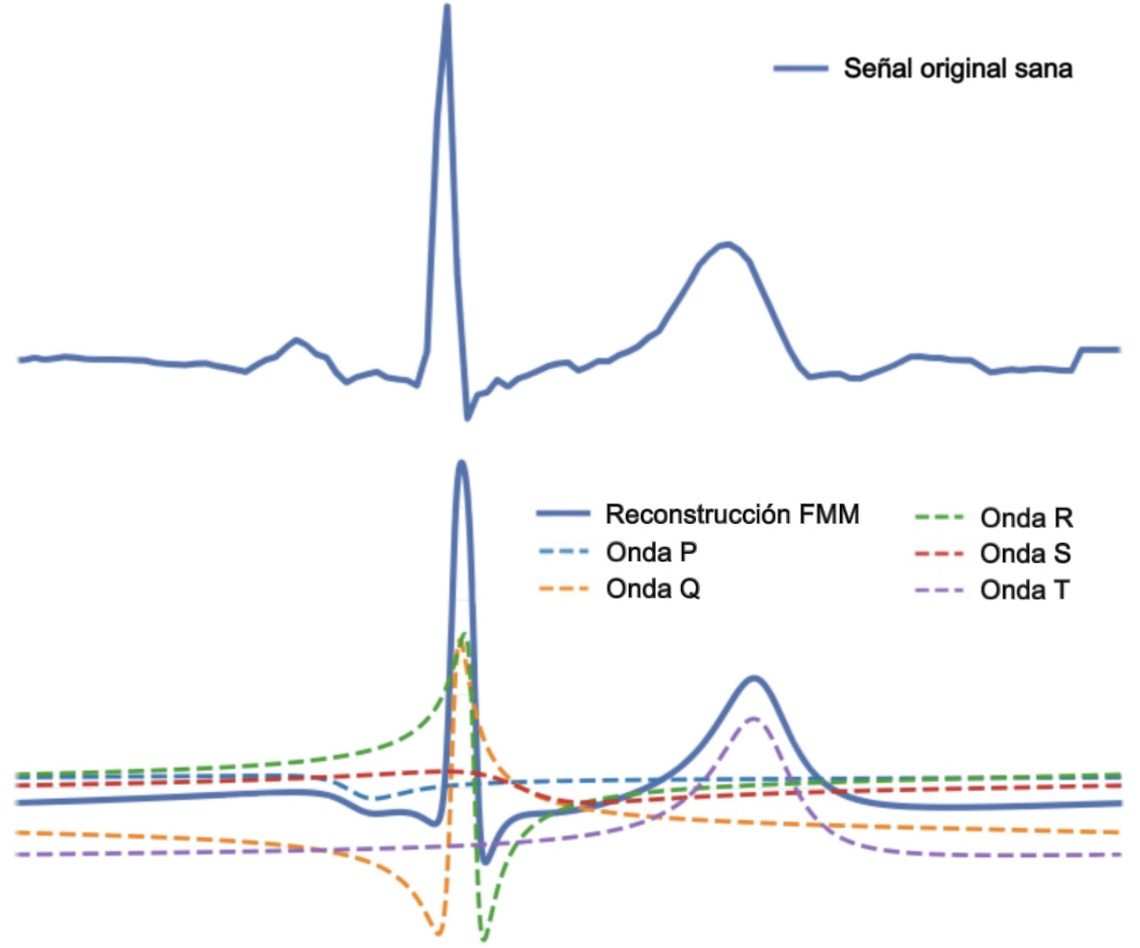
\includegraphics[width=0.9\textwidth]{ourfigures/señalesconFMM_conlabels.jpg}
    \caption{Señal de ECG y su reconstrucción mediante el modelo FMM.}
\end{figure}

\vspace{-0.30cm}
\hspace*{0.7em} Las ventanas de ECG se redimensionaron a longitud fija de 2048 muestras y cada una se normalizó mediante Z‑score utilizando las estadísticas calculadas sobre el conjunto de entrenamiento.

\vspace{0.20cm}


}




\headerbox{Referencias}{name=ref,column=0,below=details}{

\renewcommand{\section}[2]{\vskip 0.05em} % Get rid of the default "References" section title

\vspace{0.3em}

\begin{thebibliography}{9}

\bibitem{verardo2023fmmhead}
Verardo, Boman, Bruchfeld, Chiesa, Koch, Maguire Jr., y Kostic.  
\textit{FMM-Head: Enhancing Autoencoder-based ECG anomaly detection with prior knowledge}, 2023.
\vspace{0.25em}

\bibitem{jang2021unsupervised}
Jang, Kim, Lim, y Yoon.  
\textit{Unsupervised feature learning for electrocardiogram data using the convolutional variational autoencoder}, 2021.  

\end{thebibliography}
\vspace{0.22em}


\small


%\vspace{0.25cm}

%\nocite{*} % Insert publications even if they are not cited in the poster
%\small{ % Reduce the font size in this block
%\bibliographystyle{unsrt}
%\bibliography{suvs_poster} % Use sample.bib as the bibliography file

%\vspace{0.0875cm}

}





%----------------------------------------------------------------------------------------
%	Arquitectura
%----------------------------------------------------------------------------------------

\headerbox{Variational Autoencoder}{name=arquitectura,column=1}{
\hspace*{0.7em} El VAE comprime cada ventana de ECG junto con sus coeficientes FMM en un espacio latente y luego la reconstruye, de modo que el error de reconstrucción (ELBO) sirva como indicador de anomalía.
\vspace{-0.051cm}
\begin{figure}[H]
    \centering
    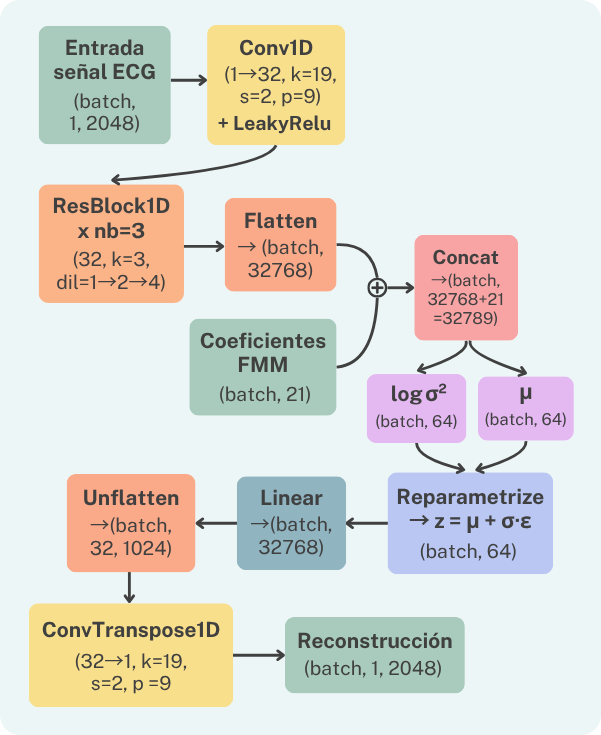
\includegraphics[width=0.9\textwidth]{ourfigures/vaearc.png}
    \caption{Arquitectura del VAE}
\end{figure}

\vspace{-5mm}

\begin{figure}[H]
    \centering
    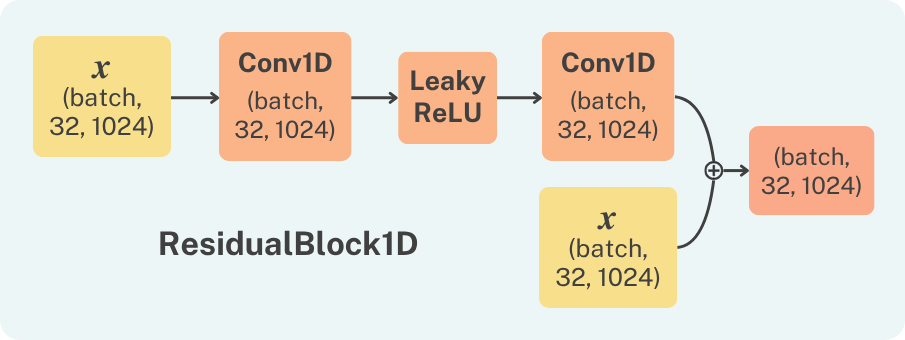
\includegraphics[width=0.78\textwidth]{ourfigures/resb1darc.png}
    \caption{Arquitectura del Resize Block 1D}
\end{figure}
\vspace{-0.4cm}

\begin{enumerate}[left=0.45em, rightmargin=0.6em]
  \item \textbf{Encoder}: recibe como entrada la señal ECG (2048 muestras) y el vector de coeficientes FMM.  
        Extrae características y proyecta en dos vectores de parámetros latentes, \(\mu\) y \(\log\sigma^2\).
  \item \textbf{Reparametrización}: a partir de \(\mu\) y \(\log\sigma^2\) se muestrea  
        \vspace{-0.3cm}
        \[
          z = \mu + \sigma \odot \epsilon,\quad \epsilon \sim \mathcal{N}(0,I).
        \]
        \vspace{-0.8cm}
  \item \textbf{Decoder}: toma \(z\) y genera la reconstrucción \(\hat{x}\) de la ventana ECG, tratando de aproximar la señal original.  
\end{enumerate}

}

%----------------------------------------------------------------------------------------
%	Data augmentation
%----------------------------------------------------------------------------------------


\headerbox{Medida de Anomalía}{name=elbo,column=2}{

\hspace*{0.5em} 4.
\vspace{-0.2cm}
\[
  \mathrm{ELBO} = -\underbrace{\mathrm{MSE}(\hat{x},x)}_{\text{reconstrucción}}
                -\beta\, \underbrace{\mathrm{KL}\bigl(q(z\mid x)\;\Vert\;\mathcal{N}(0,I)\bigr)}_{\text{regularización}}.
\]

}
  

\headerbox{XGBoost}{name=xgboost,column=2, below=elbo}{

%Toma \(\mu\) (media latente) y \(\mathit{ELBO}\) para distinguir ventanas normales de anómalas.

\hspace*{0.5em} Una vez entrenado el VAE, se extrae un vector de características $\mathbf{c} = [\boldsymbol{\mu}, e] \in \mathbb{R}^{65}$ para cada señal, donde $\boldsymbol{\mu}$ es el vector latente y $e$ el error de reconstrucción. Este vector se utiliza para entrenar un clasificador XGBoost que realiza la predicción final (\textit{Normal} vs. \textit{Anómalo}).
\vspace{-0.1cm}
%\[
%  [\mu,\;\mathrm{ELBO}] 
%  \;\longrightarrow\; \text{XGBoost} 
%  \;\longrightarrow\; \{\text{Normal},\text{Anómalo}\}
%\]
%\vspace{10cm}

\begin{figure}[H]
    \centering
    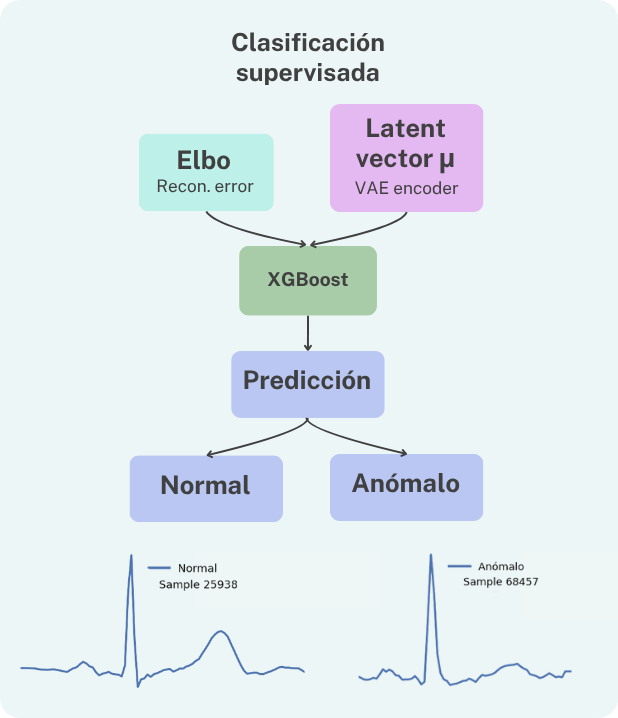
\includegraphics[width=0.9\textwidth]{ourfigures/xgboost.png}
    \caption{Clasificador del XGBoost}
\end{figure}




}



\headerbox{Conclusiones y Trabajo a Futuro}{name=conclu,column=2,below=xgboost}{
\vspace{0.1cm}
\begin{itemize}[left=0.45em, rightmargin=0.6]
    \item El pipeline VAE + XGBoost logró detectar anomalías en ECG con alta precisión.
    \item El uso de coeficientes FMM aportó conocimiento morfológico muy útil al modelo.
    \item Se observó un trade-off entre precisión y recall, priorizando señales claras.
    \item A futuro, podrían incorporarse mecanismos de atención o datos sintéticos.

\vspace{0.55cm}

\end{itemize}

}





%----------------------------------------------------------------------------------------
%	Resultados
%----------------------------------------------------------------------------------------

\headerbox{Resultados}{name=resultados,column=1,span=2, below=arquitectura}{


%\vspace{0.5em}

\begin{center}

\includegraphics[width=0.3\textwidth]{ourfigures/matconfval2.png}
\hspace{2em}

\includegraphics[width=0.3\textwidth]{ourfigures/matconftest2.png}

\vspace{0.3em}
\small
Matrices de confusión: validación (izq.) y test (der.)
\end{center}

\vspace{-0.25em}

Los resultados numéricos del modelo final se resumen en la Tabla. Se observa un rendimiento general alto, con un AUC superior a 0.91 en el conjunto de prueba.
\vspace{-0.1cm}

\small
\begin{center}
\begin{tabular}{lcc}
\toprule
\textbf{Métrica} & \textbf{Validación} & \textbf{Test} \\
\midrule
AUC-ROC   & 0.9235 & 0.9151 \\
Precision & 0.8780 & 0.9207 \\
Recall    & 0.8276 & 0.7084 \\
F1-score  & 0.8521 & 0.8007 \\
Accuracy  & 0.8563 & 0.8237 \\
\bottomrule
\end{tabular}
\end{center}


}







% \begin{textblock*}{7cm}(3cm, 34.5cm) % 5cm width, (3cm, 4cm) is the position on the page
%     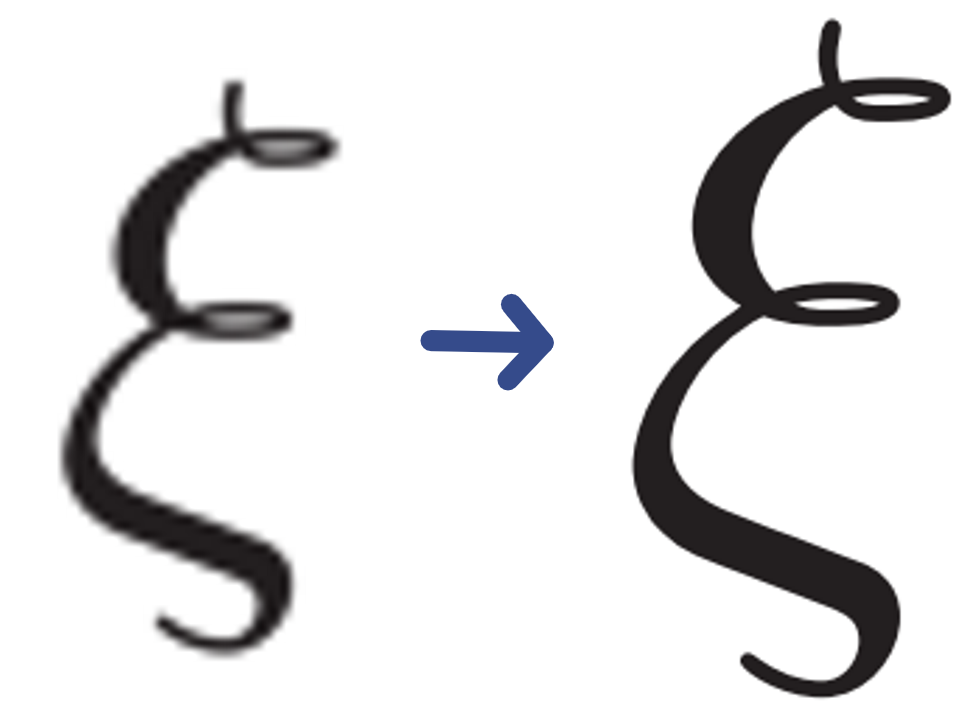
\includegraphics[width=1.5cm]{figures/xi.png} % Include the image at the specified position
% \end{textblock*}

%----------------------------------------------------------------------------------------
% Ajustes del resto del documento
%----------------------------------------------------------------------------------------

% No olvides reemplazar las imágenes y referencias en el código según corresponda.

\end{poster}

\end{document}